\section{Goal}

\begin{frame}{Goal}
  Ease learning functional programming by means of an interactive
  interface based on a tangible block-world with augmented reality
  and software feedback.
  \vfill
  \textsf{Tags}: functional programming, tangible user-interface,
  block world, augmented reality, software feedback
\end{frame}


%***
%***
\section{Recursion Difficulties}

\begin {frame} {The effect of dynamic copies model in teaching recursive programming}
  \footnotetext{Paper: 1998 - Ming Puu Chen}
  
  Cognitive load theory:
  
  \begin{enumerate}
  \item People have a very limited working memory which can hold and process
    only a few items of information at a time.
  \item People have an extensive long-term memory that is effectively
    unlimited in size.
  \end{enumerate}
\end{frame}

\begin{frame}{The case of bad cases}
  \footnotetext{Paper: 2002 - Bruria Haberman and Haim Averbuch}
  
  Students have difficulties in identifying base cases:
  
  \begin{itemize}
  \item Handle redundant base cases.
  \item Ignore boundary values and degenerated cases.
  \item Avoid out-of-range values.
  \item May not even define any base cases.
  \end{itemize}
\end{frame}

\begin{frame}{Mental models of recursion revisited}
  \footnotetext{Paper: 2006 - Ian Sanders, Vashti Galpin, and Tina Gotschi}
  
  There are different kinds of mental models on how students understand
  recursion.
  
  \begin{itemize}
  \item Copies Model
  \item Looping Model
  \item Active Model
  \item Step Model
  \item Return Value Model
  \item Magic or Syntactic Model
  \item Algebraic Model
  \item Odd Model
  \end{itemize}
\end{frame}


%***
%***
\section{Recursion Didactics}

\begin{frame}{Experimental evaluation of teaching recursion in a video game}
  \footnotetext{Paper: 2009 - Amanda Chaffin, Katelyn Doran, Drew Hicks, and Tiffany Barnes}
  
  EleMental: The Recurrence; is a game that allows students to learn about
  recursion through depth-first search of a binary tree.
  \medskip
  
  The game is designed to maximize transfer of learning to writing real
  programs, while also providing interactive visualizations.
  \medskip
  
  Measure the impact of the game on learning and on attitudes toward
  educational games.
  \medskip
\end{frame}

\begin{frame} {Ele, A programmable Avatar}
  The overall design of the game involves completing three
  programming puzzles, helped by Ele, a programmable avatar.
  \medskip
  
  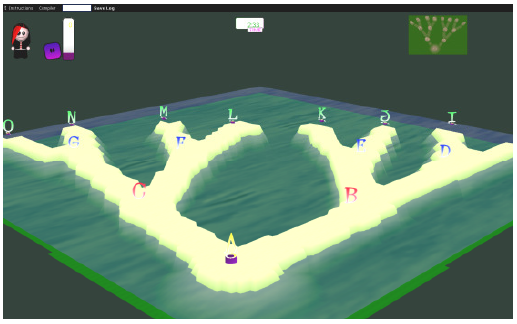
\includegraphics[scale=0.7]{img/ele.png}
\end{frame}

\begin{frame}{A graphical technique for describing recursion}
  \footnotetext{Paper: 1976 - Glenn A. Jackson}
  
  Method of describing recursive procedure calls that utilizes a
  form of self-generating state diagram.
  \medskip
  
  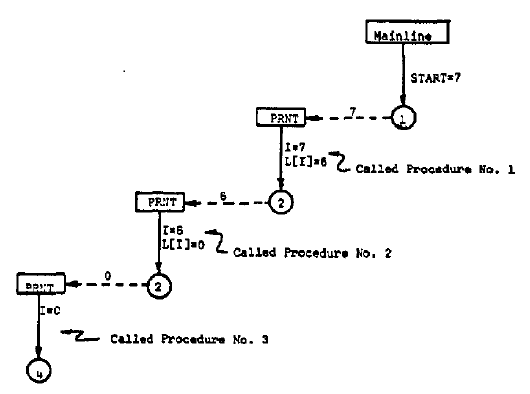
\includegraphics[scale=0.5]{img/visualizing_recursion.png}
\end{frame}

\begin{frame} {Why structural recursion should be taught before arrays}
  \footnotetext{Paper: 2005 Kim B. Bruce, Andrea Danyluk, and Thomas Murtagh}
  
  Early presentation of recursive structures provides the opportunity
  to reinforce the fundamentals of defining and using classes
  and prepares students to appreciate the reasons to use classes
  to encapsulate access to other data structures.
\end{frame}


%***
%***
\section{TUIs used at Learning}

\begin{frame} {Do tangible interfaces enhance learning}
  \footnotetext{Paper: 2007 - Paul Marshall}

  The use of physical materials per se could help on the
  process of learning.
  
  \begin{itemize}
  \item Using material change the nature of the knowledge
    because perception and cognition are closely interlinked.
  \item 3D forms might be perceived and understood more readily
    through haptic or other tangible representations than
    through visual representation alone.
  \item In young children manipulation of concrete
    physical objects helps to support and develop thinking.
  \end{itemize}
\end{frame}

\begin{frame} {Designing tangible programming languages for classroom use}
  \footnotetext{Paper: 2007 - Michael S. Horn and Robert J.K. Jacob}
  
  With Tern, programmers connect wooden blocks shaped like jigsaw
  puzzle pieces to form flow-of-control chains.
  \medskip

  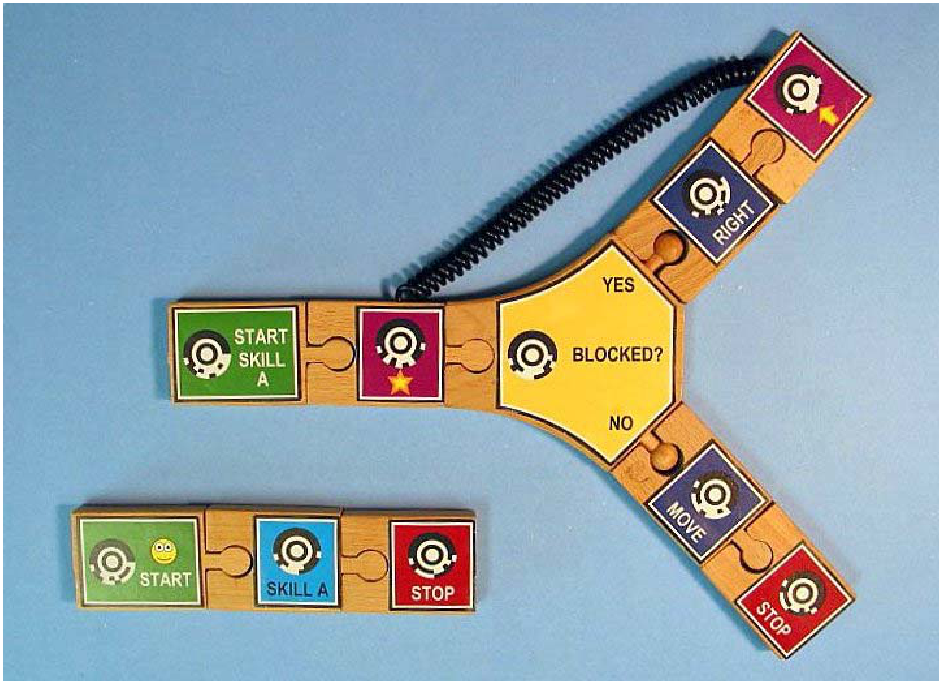
\includegraphics[scale=0.3]{img/tern.png}
\end{frame}

\begin{frame} {Using artoolkit markers to build tangible prototypes}
  \footnotetext{Paper: 2005 - Eva Hornecker and Thomas Psik}
  
  As a work-around for a class on experimental prototyping of
  tangible appliances we utilized the ARToolKit that tracks
  optical markers.
  \medskip
  
  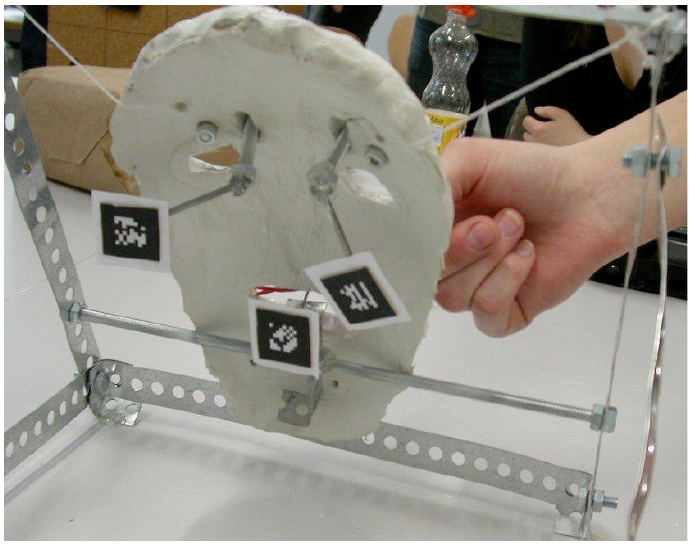
\includegraphics[scale=0.4]{img/artoolkit_prototyping.png}
\end{frame}


%***
%***
\section{Transfer of Training}

\begin{frame} {Can direct manipulation lower the barrier to computer programming}
  \footnotetext{Paper: 2006 - Christopher D. Hundhausen, Sean Farley, and Jonathan Lee Brown}
  
  Direct manipulation programming environments provides concrete visual
  representations on which to operate.
  \medskip
  
  In many cases the learning goal of the novice is to be able ultimately to
  program in conventional textual languages.
\end{frame}

\begin{frame} {The Interface}
  New direct manipulation programming interface for
  ALVIS Live!, a novice programming environment.
  \medskip
  
  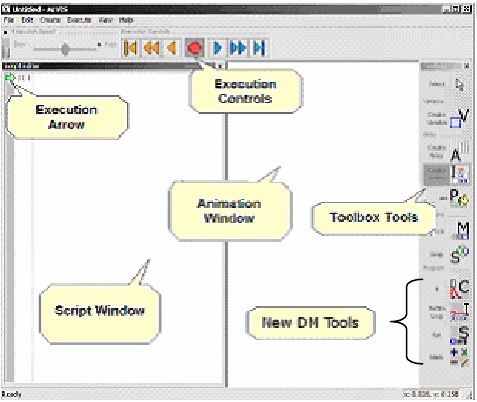
\includegraphics[scale=0.6]{img/alvis.png}
\end{frame}

\begin{frame} {The experiments}
  Conducted an experimental study that compared the programming
  outcomes from the new direct manipulation interface to those
  from the textual programming interface.
  \medskip
  
  Found that the direct manipulation interface not only led
  to significantly better initial programming outcomes, but
  also to significant positive transfer to the textual interface.
\end{frame}

